\section{Konzeption der Programmieraufgabe: Das \enquote{Garden-Simulator}-Framework}

Nach dem persönlichen Fragebogen und nachdem die Entwicklungsumgebung bereitsteht, soll die Programmieraufgabe von den Studierenden bearbeitet werden. Dieses Kapitel behandelt den Aufbau und Hintergrund des Python-Programms \anf{Garden-Simulator}, die Aufgabenerstellung sowie die erwarteten Lösungen und die Testumgebung.

\subsection{Der \anf{Garden-Simulator}}
Der \textit{Garden-Simulator} ist eine didaktische Python-Applikation, die die Studierenden im Zuge der einstündigen Studie adaptieren sollen. Das Programm wird im folgenden Kapitel anhand der \textit{4+1 View Model}-Methode nach \textcite{kruchten_41_1995} erläutert.

\subsubsection{Logische Architektur}
\textcite[S.~3]{kruchten_41_1995} spircht im Bereich der logischen Architektur von der objektorientierten Zerlegung (Dekomposition) der Problemstellung bzw. Anforderung in ihre zentralen Aspekte als Objekte oder Objektklassen. Dabei kommen die Prinzipien der Abstraktion, Kapselung und Vererbung zum Einsatz. Diese Zerlegung dient nicht nur der funktionalen Analyse, sondern auch dazu, gemeinsame Mechanismen und Entwurfselemente in den verschiedenen Teilen des Systems zu identifizieren \parencite[S.~3]{kruchten_41_1995}.

\begin{figure}[htbp]
  \centering
  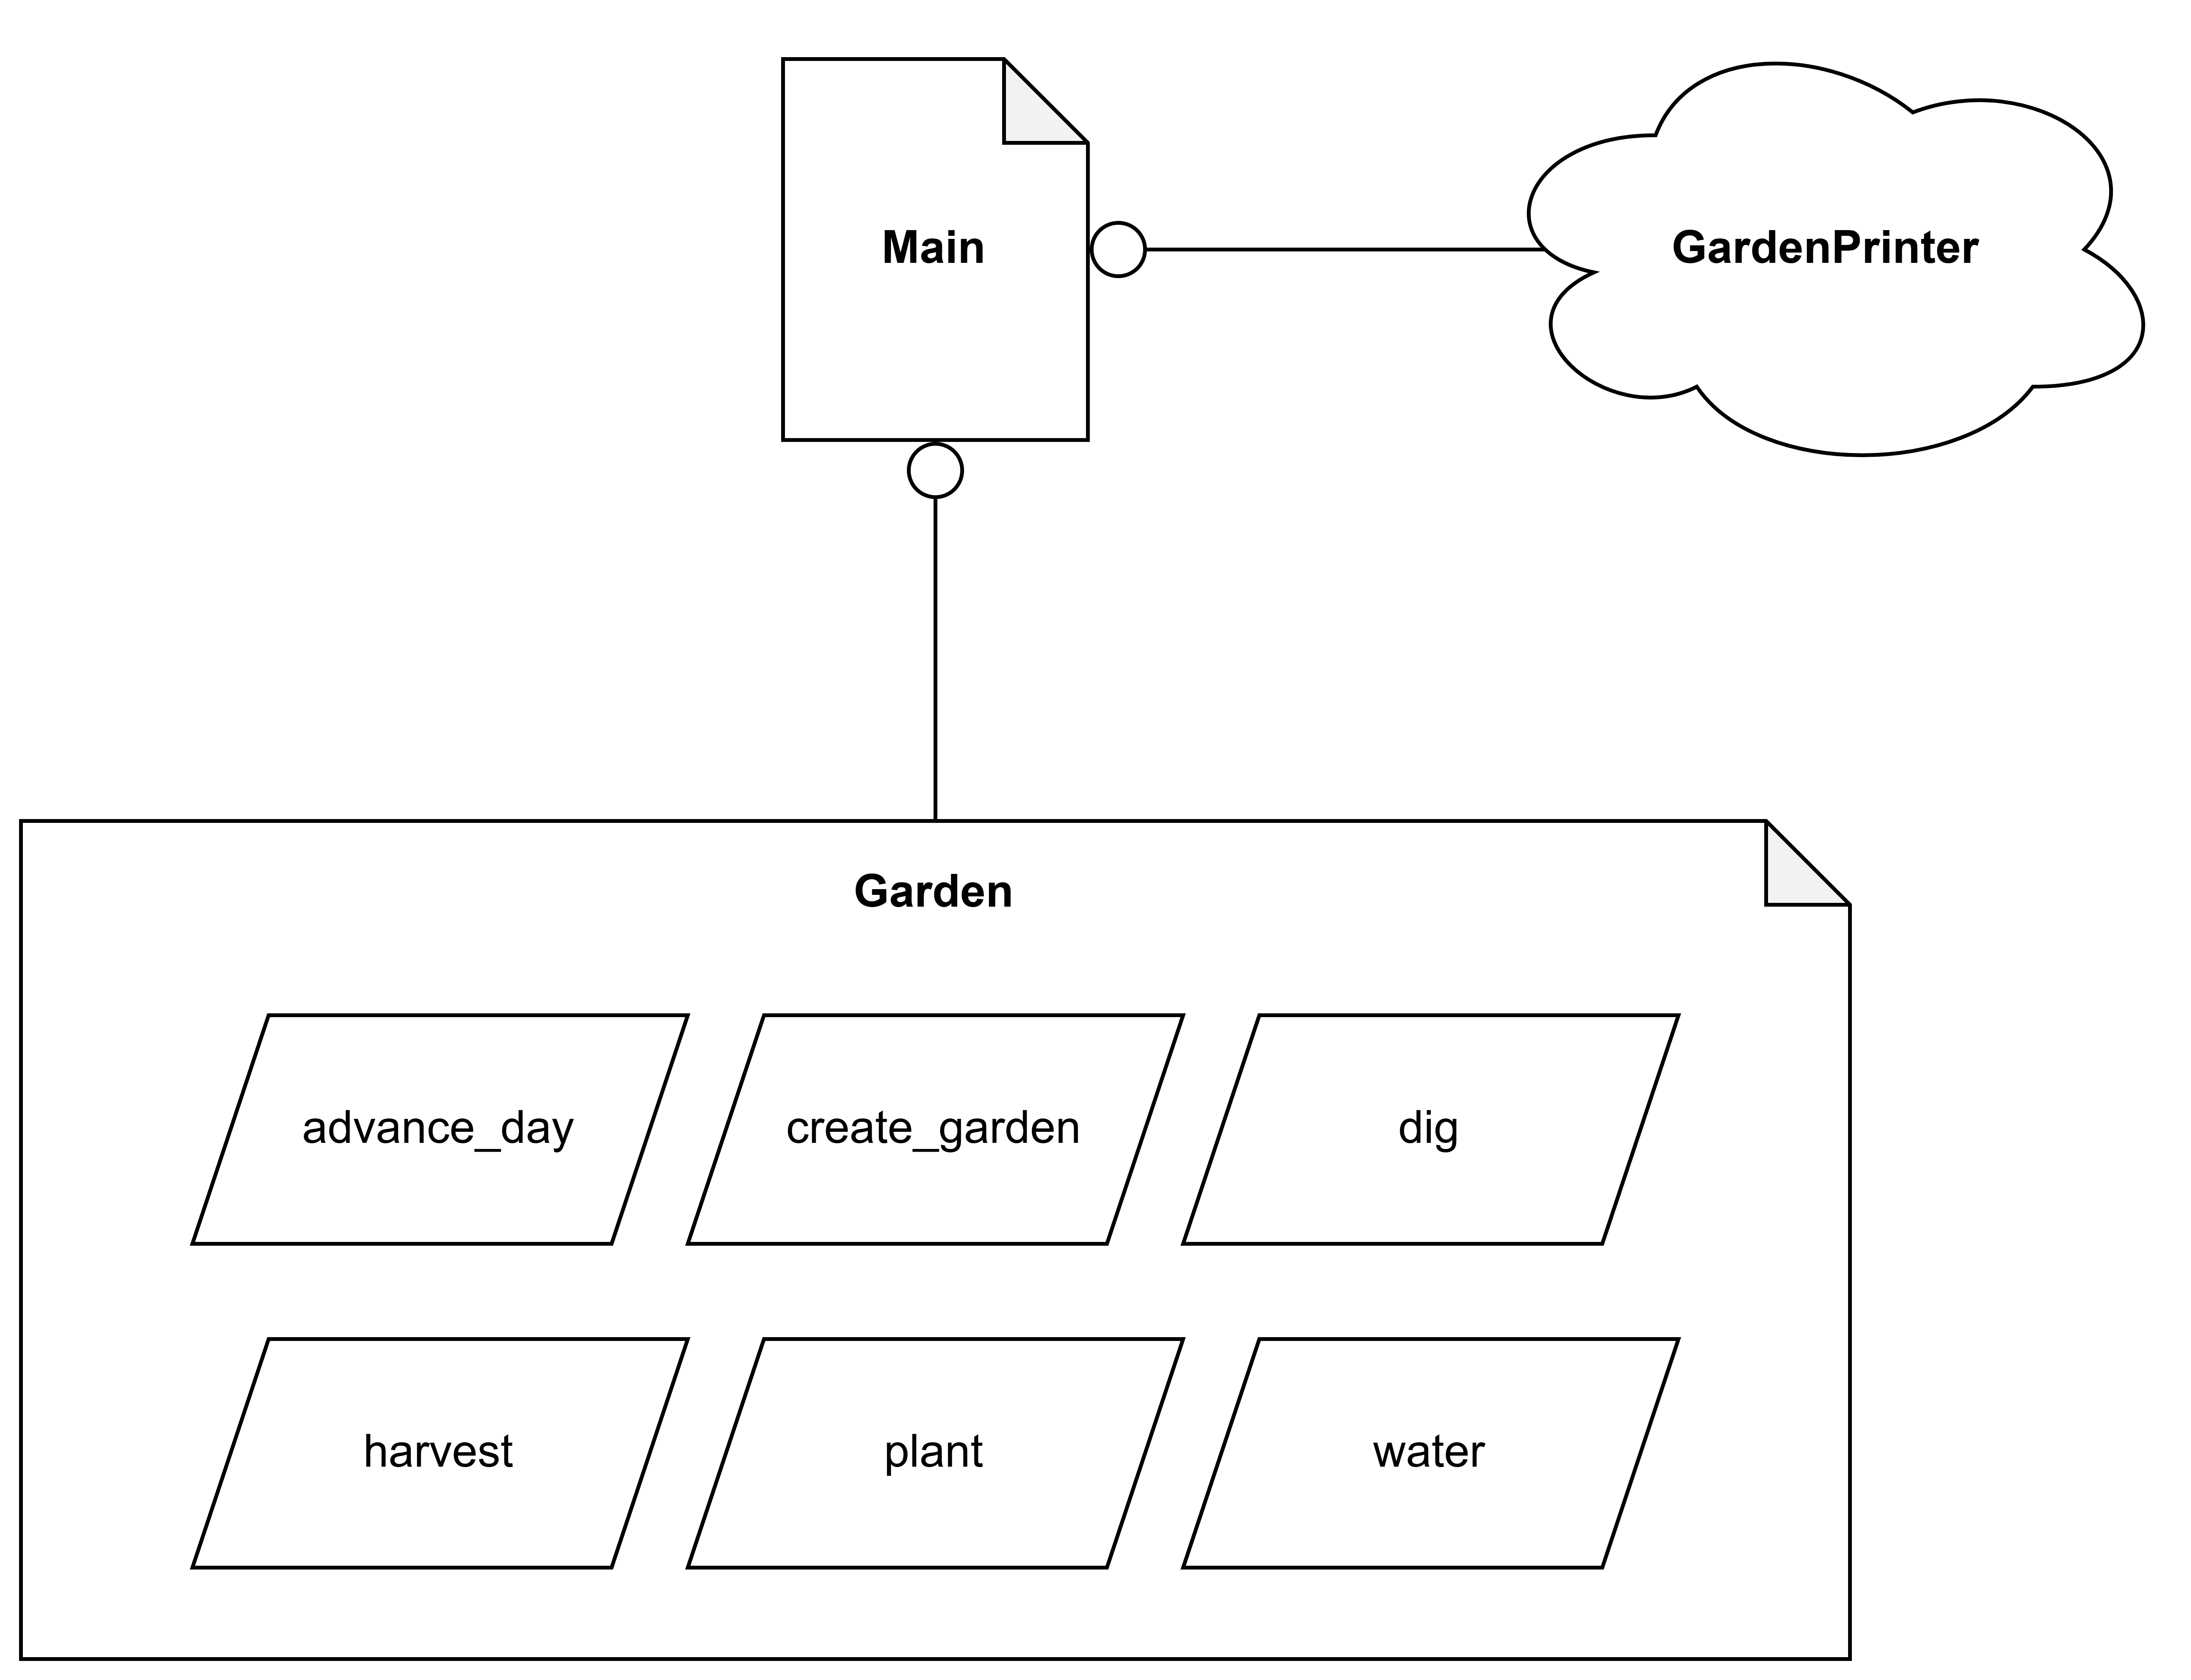
\includegraphics[width=0.9\textwidth]{00_figures/logical-view-v2.png}
  \caption{Logik-Ansicht des Garden Simulators nach \textcite[S.~4]{kruchten_41_1995}}
  \label{fig:logik-view}
\end{figure}

Im \textit{Garden-Simulator} wurde aufgrund der didaktischen Ausrichtung und des einstündigen Zeitrahmens mit Absicht auf eine umfangreiche Klassen-Struktur verzichtet. Einzig, wie es in Abb. \ref{fig:logik-view} zu erkennen ist, wird für die Ausgabe des Spielfeldes im Terminal eine Klasse namens \textit{Garden-Printer} verwendet. Diese müssen die Studierenden aber nicht adaptieren. Zusätzlich zur Ausgabe-Klasse gibt es die Datei \textit{Garden}, in der Funktionen wie \texttt{advance\_day} oder \texttt{dig} implemtiert sind, die neben den anderen Funktionen dieser Datei zur Kernlogik des Programms zählen. Beide, \textit{GardenPrinter} und \textit{Garden}, werden in \textit{Main} eingebunden, welche als Eintrittspunkt gilt und zur Kommando-Verwaltung verwendet wird. Änderungen am Programmcode sind von den Studierenden in den Elementen \textit{Garden} sowie \textit{Main} durchzuführen.

\subsubsection{Prozessuale Architektur}
Bei der Prozessarchitektur geht es nach \textcite[S.~4]{kruchten_41_1995} um die Einordnung der wichtigsten Abstraktionen aus der logischen Sicht in die Prozess-Sicht, also die Frage, in welchem Abschnitt eine Operation eines Objekts ausgeführt wird. Weiters geht es um die Darstellung von gleichzeitgen oder wiederkehrenden Abläufen, Verteilung sowie Systemintegrität und Fehlertoleranz \parencite[S.~4]{kruchten_41_1995}.

Ein Prozess wird definiert als eine Gruppierung von Tasks, die eine ausführbare Einheit bilden. Prozesse können z.B. repliziert werden, um die Verarbeitungslast zu verteilen oder die Verfügbarkeit zu erhöhen. Ein Task ist ein unabhängiger und planbarer Ausführungsstrang auf einem Verarbeitungsknoten. Dabei werden eindeutig adressierbare, architektonisch relevante Haupttasks von unterstützenden Nebentasks unterschieden. Letztere übernehmen beispielsweise zyklische Aktivitäten, Pufferung oder die Behandlung von Zeitüberschreitungen. Haupttasks kommunizieren über Mechanismen wie z.B. synchrone und asynchrone nachrichtenbasierte Kommunikation, entfernte Prozeduraufrufe oder Event-Broadcasts \parencite[S.~4-5]{kruchten_41_1995}.

In Abb. \ref{fig:process-view} sind die Prozesse dargestellt, die im \gs vorzufinden sind. Der Einstiegspunkt in das Programm erfolgt durch den Prozess \textit{Programmstart}. Hier werden

\begin{figure}[htbp]
  \centering
  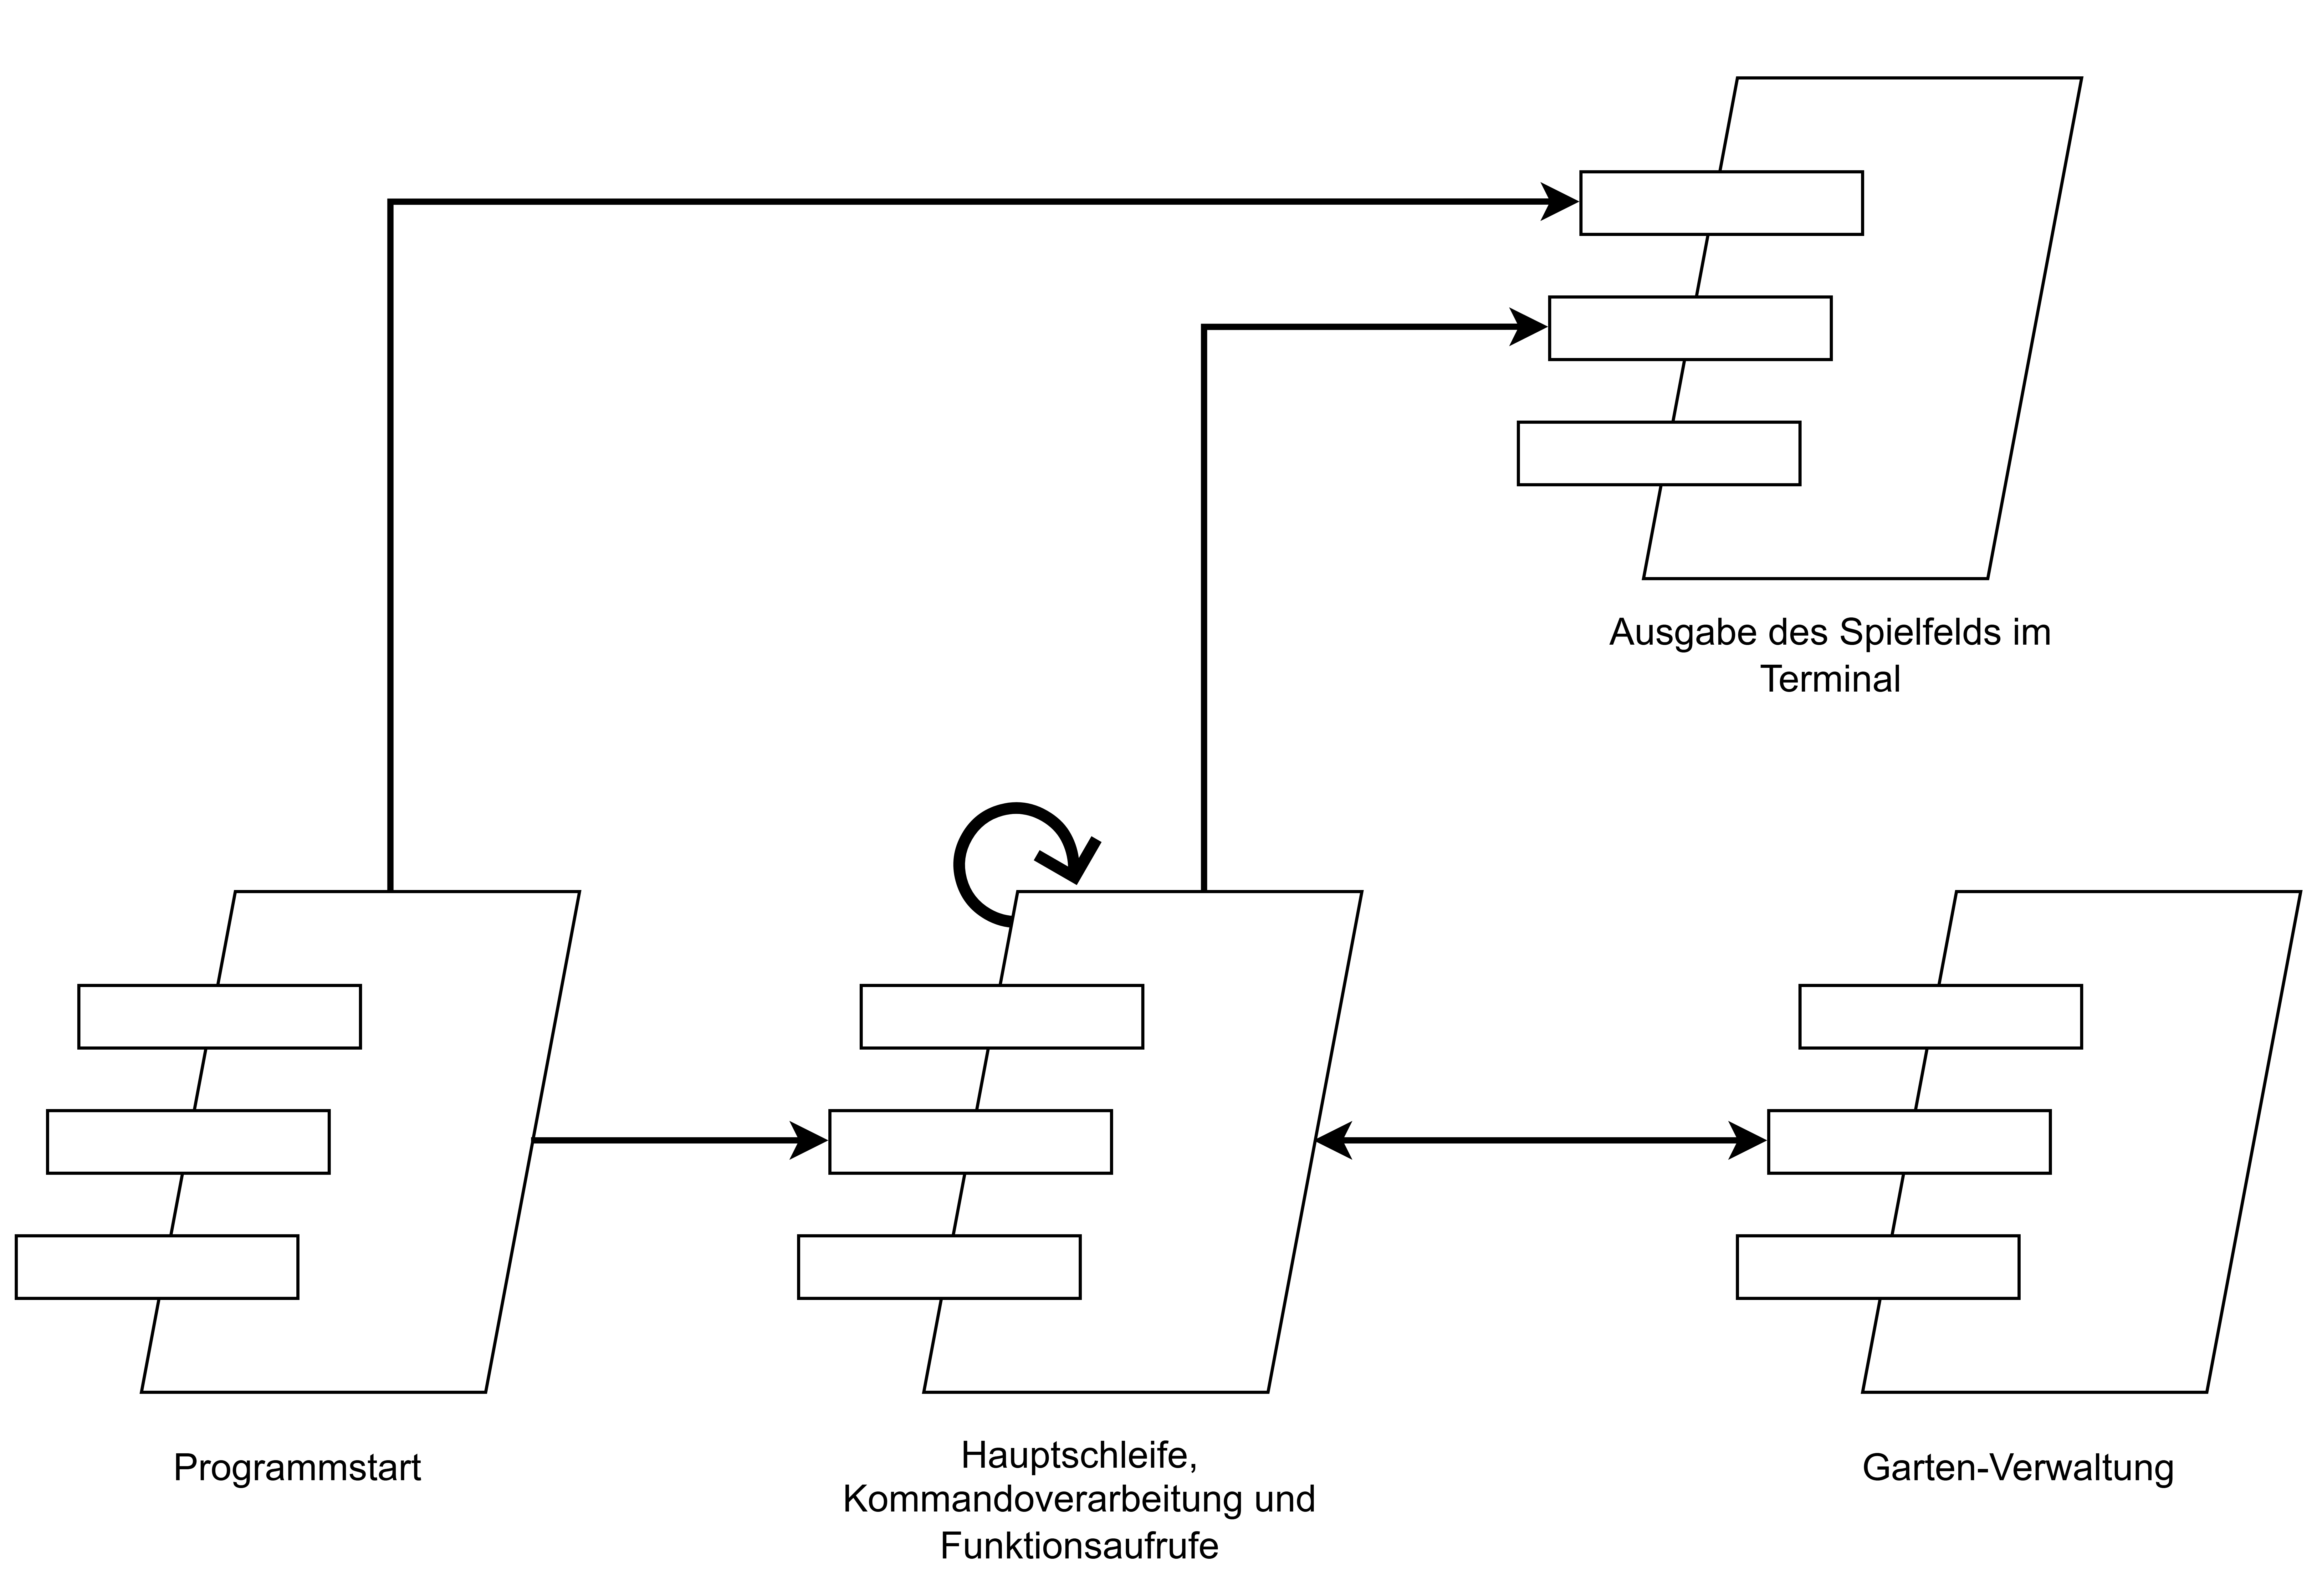
\includegraphics[width=0.9\textwidth]{00_figures/process-view.png}
  \caption{Prozess-Ansicht des Garden Simulators nach \textcite[S.~5-6]{kruchten_41_1995}}
  \label{fig:process-view}
\end{figure}


\subsubsection{Entwicklungs-Architektur}\label{cha:entwicklungs-architektur}

Die Entwicklungs-Architektur beschreibt nach \textcite[S.~6]{kruchten_41_1995} die Organisation der Softwaremodule in ihrer Entwicklungsumgebung. Im Mittelpunkt stehen die modulare Aufteilung sowie deren Import- und Exportbeziehungen. Diese Sicht berücksichtigt insbesondere die einfache Weiterentwicklung, Wiederverwendbarkeit und Verteilung der Entwicklungsaufgaben. Kruchten empfiehlt dazu eine Gliederung in Schichten mit klar definierten Zuständigkeiten, wobei Abhängigkeiten innerhalb derselben oder zu darunterliegenden Schichten verlaufen sollen \parencite[S.~7]{kruchten_41_1995}.

Im \textit{Garden-Simulator} sind die drei Hauptkomponenten \texttt{main.py}, \texttt{garden.py} und \texttt{cli\_view.py} gemeinsam im Projektverzeichnis vorzufinden. Aufgrund der didaktischen Ausrichtung und der damit erforderlichen Reduktion erfolgt keine weitere Aufteilung in Subsysteme. Wie in Abb.~\ref{fig:development-view} dargestellt, bindet \texttt{main.py} sowohl die Funktionen aus \texttt{garden.py} als auch die Klasse \texttt{GardenPrinter} aus \texttt{cli\_view.py} ein. Es übernimmt dabei die Verarbeitung der Eingaben und verbindet so die Simulationslogik mit der Darstellung. Die beiden eingebundenen Module importieren sich einander nicht und haben keine Importabhängigkeit zu \texttt{main.py}. Die Daten aus dem Garten wie z.B. welche Pflanze auf einem Feld platziert ist, werden ihnen als Funktions- bzw. für den \texttt{GardenPrinter} als Methodenparameter übergeben.

\begin{figure}[htbp]
  \centering
  \setlength{\unitlength}{1mm}
  \begin{picture}(120,76)
    \put(0,66){\framebox(45,10){\texttt{main.py}}}
    \put(75,66){\framebox(45,10){\texttt{cli\_view.py}}}
    \put(0,0){\framebox(45,46){}}
    \put(0,36){\makebox(45,10){\texttt{garden.py}}}
    \put(0,36){\line(1,0){45}}
    \put(0,0){\makebox(45,36){\small\shortstack[l]{
      \texttt{create\_garden()}\\
      \texttt{dig()}\\
      \texttt{plant()}\\
      \texttt{water()}\\
      \texttt{advance\_day()}\\
      \texttt{harvest()}
    }}}
    \put(75,30){\framebox(45,10){\texttt{test\_runner.py}}}
    \put(45,71){\vector(1,0){30}}
    \put(22,66){\vector(0,-1){20}}
    \put(75,35){\vector(-1,0){30}}
    \put(75,35){\vector(-1,1){31}}
  \end{picture}
  \caption[Entwicklungs-Ansicht des Garden-Simulators]{Entwicklungs-Ansicht des Garden-Simulators. Die Pfeile zeigen vom importierenden zum eingebundenen Modul. Der Testrunner importiert dynamisch über \texttt{importlib}. Darstellung nach \textcite[S.~6--7]{kruchten_41_1995}.}
  \label{fig:development-view}
\end{figure}

Das Modul \texttt{garden.py} stellt die Funktionen zur Bearbeitung des Gartens bereit und verwendet für die Erntelogik der Planze Tomate die Module \texttt{pathlib} und \texttt{datetime} aus der Python-Standardbibliothek. Die Datei \texttt{cli\_view.py} stellt die Klasse \texttt{GardenPrinter} zur Verfügung, die die übergebenen Daten des Garten als Raster aufbereitet und im Terminal ausgibt. Diese Aufteilung nach Zuständigkeiten erleichtert es, Änderungen gezielt einem Modul zuzuordnen, was nicht zuletzt ein primärer Faktor für die Planung der Aufgaben war, denn die Studierenden sollten sich z.B. mit der visuellen Darstellung des Rasters nicht beschäftigen. Eine Ausnahme bildet ein \texttt{print}-Befehl in \texttt{garden.py}, der bei der Ernte erzeugt wird. Dieser ist jedoch von den Studierenden anzupassen und konnte deshalb in \texttt{garden.py} bleiben.

Ergänzt werden die Hauptmodule durch \texttt{test\_runner.py}, die Dokumentationsdateien \texttt{README.md} und \texttt{Aufgaben.md} sowie ein \texttt{Makefile}. Der Testrunner prüft den Quelltext von \texttt{main.py} und lädt die Module \texttt{garden.py} und \texttt{main.py}. Dieser wird in Abschnitt \ref{cha:test-runner} detailliert erklärt. Das \texttt{Makefile} fasst die Aufrufe zum Starten der Anwendung und der Tests zusammen. Für die Bearbeitung der Programmieraufgabe sind Änderungen in \texttt{main.py} und \texttt{garden.py} vorgesehen. Die Darstellung und die Tests werden bereitgestellt. Damit unterstützt die Modulaufteilung, wie im letzten Absatz erwähnt, die Eingrenzung der Entwicklungsaufgaben im einstündigen Zeitrahmen der Studie.

\subsubsection{Physikalische Architektur}

Die physikalische Architektur behandelt nach \textcite[S.~8]{kruchten_41_1995} die Zuordnung der Software zu den verfügbaren Hardwareknoten, genannt \textit{nodes}. Dabei werden insbesondere Eckpunkte wie Verfügbarkeit, Fehlertoleranz, Leistung und Skalierbarkeit betrachtet. Des Weiteren können unterschiedliche Zuordnungen für Entwicklung, Tests und den tatsächlichen Betrieb beschrieben werden. Für den \textit{Garden-Simulator} werden deshalb zwei Ausführungsvarianten unterschieden: die lokale Ausführung und die Ausführung in GitHub Codespaces während der Prüfungssituation.

In der lokalen Variante werden, wie in Abb. \ref{fig:physical-view} a) gezeigt, sämtliche Bestandteile des \textit{Garden-Simulators} einem lokalen Rechner zugeordnet. Die Anwendung wird im Projektverzeichnis mit \texttt{python main.py} gestartet. Der dabei ausgeführte Python-Prozess lädt die Module wie in \ref{cha:entwicklungs-architektur} beschrieben. Diese werden nicht als eigenständige Prozesse gestartet. Die Interaktion erfolgt über die Standardeingabe und Standardausgabe des Terminals. Abb.~\ref{fig:garden-sim} zeigt die Ausgabe nach Ausführung des \texttt{show}-Befehls. Der Benutzer benötigt für diese Ausführungsvariante keine Netzwerkverbindung.

\begin{figure}[htbp]
  \centering
  \small
  \setlength{\unitlength}{1mm}
  \begin{picture}(140,158)
    \put(0,118){\framebox(140,40){}}
    \put(0,150){\makebox(140,8){\textbf{a) Lokaler Rechner}}}
    \put(5,138){\framebox(60,9){Terminal: Ein- und Ausgabe}}
    \put(35,138){\vector(0,-1){6}}
    \put(35,132){\vector(0,1){6}}
    \put(5,122){\framebox(60,10){\shortstack{Python-Prozess\\\texttt{main.py} oder \texttt{test\_runner.py}}}}
    \put(65,127){\vector(1,0){15}}
    \put(80,122){\framebox(55,25){\shortstack{Lokales Dateisystem:\\Projektdateien und\\\texttt{harvests/tomato.txt}}}}

    \put(0,82){\framebox(140,25){}}
    \put(0,98){\makebox(140,9){\textbf{b) Prüfungssituation: lokaler Rechner}}}
    \put(10,86){\framebox(120,9){Browser mit VS-Code-Webclient}}
    \put(70,82){\vector(0,-1){10}}
    \put(70,72){\vector(0,1){10}}
    \put(76,74){\makebox(40,6)[l]{Internetverbindung}}

    \put(0,0){\framebox(140,72){}}
    \put(0,63){\makebox(140,9){\textbf{b) Prüfungssituation: GitHub Codespace}}}
    \put(5,21){\framebox(130,39){}}
    \put(5,52){\makebox(130,8){\textbf{Devcontainer: Python 3}}}
    \put(10,40){\framebox(120,9){Remote Terminal: Ein- und Ausgabe}}
    \put(70,40){\vector(0,-1){4}}
    \put(70,36){\vector(0,1){4}}
    \put(10,25){\framebox(120,11){\shortstack{Python-Prozess: \texttt{main.py} oder \texttt{test\_runner.py}\\Module: \texttt{garden.py} und \texttt{cli\_view.py}}}}
    \put(70,25){\vector(0,-1){9}}
    \put(5,3){\framebox(130,13){\shortstack{Persistenter Workspace (in den Devcontainer eingebunden)\\Projektdateien und \texttt{harvests/tomato.txt}}}}
  \end{picture}
  \caption[Physikalische Ansicht des Garden-Simulators]{Physikalische Ansicht des Garden-Simulators: lokale Ausführung (a) und Prüfungssituation mit GitHub Codespaces (b). Eigene Darstellung nach \textcite[S.~8]{kruchten_41_1995} und der Codespaces-Infrastruktur \parencite{github_codespaces_deep_dive}.}
  \label{fig:physical-view}
\end{figure}

In der Prüfungssituation wird hingegen GitHub Codespaces mit einem Devcontainer verwendet. Wie in Abb.~\ref{fig:physical-view} b) dargestellt, fungiert der lokale Rechner dabei als Zugang zur VS-Code-Webclient Entwicklungsumgebung. Der Devcontainer läuft auf einer von GitHub bereitgestellten virtuellen Maschine (VM) \parencite{github_codespaces_deep_dive}. Die Eingaben und Ausgaben werden über die Netzwerkverbindung zwischen dem lokalen Rechner und dem Codespace übertragen. Die Ausführung der Anwendung und der Tests findet im Devcontainer statt. GitHub Codespaces wurde aus zweierlei Gründen als Lösung für die Prüfungssituation herangezogen. Einerseits weil es durch den Devcontainer für jeden Student/jede Studentinn diesselbe Umgebung bereitstellt. Andererseits kann durch die Konfigurationsdatei die VS-Code Entwicklungsumgebung vorab eingestellt werden und so diverse AI-Features deaktiviert werden, was für den Versuch von zentraler Wichtigkeit war.

Die im letzten Absatz angesprochene Konfigurationsdatei befindet sich in der unter \path{.devcontainer/devcontainer.json} des Projektsverzeichnisses. Dort festgelegt sind das Container-Image (\path{mcr.microsoft.com/devcontainers/python:3}) und die VS-Code-Erweiterungen sowie Editor-Einstellungen. Die voreingestellten Erweiterungen sind \texttt{ms-python.python}, \texttt{ms-python.vscode-pylance} und ein Markdown-Previewer namens \texttt{bierner.markdown-preview-github-styles}. Um eine KI-freie Entwicklungsumgebung garantieren zu können, wurden VS-Code-Einstellungen gesetzt wie z.B. \texttt{chat.disableAIFeatures : true}, um KI-Chat-Erweiterungen, oder \texttt{editor.inlineSuggest.enabled : false}, um zeilenweise KI-Codevervollständigung auszuschalten. Zudem wurde der Standardformatierer (\texttt{editor.defaultFormatter}) auf \texttt{NULL} gesetzt sowie \texttt{editor.formatOnSave} ausgeschalten, damit diese automatischen Formatierungshilfen die Kategorie \anf{Layout \& Formatierung} des Bewertungsraster (siehe Abschnitt \ref{cha:bewertungsraster}) nicht beeinflussen. 

Das aktuelle Garten-Spielfeld und der Tageszähler, der mit \texttt{advance\_day} erhöht werden kann, werdenim Arbeitsspeicher des ausführenden Python-Prozesses gespeichert und bei einem Neustart der Anwendung neu angelegt. Dauerhaft gespeichert wird eine Ernte-Log-Datei für Tomaten: Die Funktion \texttt{create\_tomato\_\allowbreak harvest\_file} legt, wenn nicht vorhanden, das Verzeichnis \texttt{harvests} an und fügt eine Log-Zeile in die Datei \texttt{tomato.txt} ein. Beim vorgesehenen Start im Projektverzeichnis entsteht somit die Datei \texttt{harvests/tomato.txt} innerhalb des Projekts. Lokal liegt diese Datei auf dem verwendeten Rechner (siehe Abb. \ref{fig:physical-view} (a) Lokales Dateisystem), in der Prüfungssituation im Workspace des Codespaces (siehe Abb. \ref{fig:physical-view} (b) Persistenter Workspace). GitHub bindet das Repository im Pfad \path{/workspaces} in den Devcontainer ein und die dort gespeicherten Dateien bleiben beim Stoppen und erneuten Starten des Codespaces erhalten \parencite{github_codespaces_deep_dive}.

Der Grund für die Erstellung eines Ernte-Logs für Tomaten ist die erste Aufgabe (siehe Abschnitt \ref{cha:Aufgabenstellung}). Um diese Aufgabe erfolgreich zu absolvieren, müssen die Studierenden das Python-Programm über die Kommandozeile kennenlernen und mindestens einen Ernte-Zyklus für eine Tomate durchspielen. Am Ende des Zyklus wird die \texttt{tomato.txt} erstellt, was für den Test-Runner der Indikator dafür ist, dass die erste Aufgabe erfolgreich abgeschlossen wurde. Der Aufruf des Test-Runners mittles \texttt{python test\_runner.py} startet einen beiden Umgebungen einen eigenen Python-Prozess.

\begin{figure}[htbp]
  \centering
  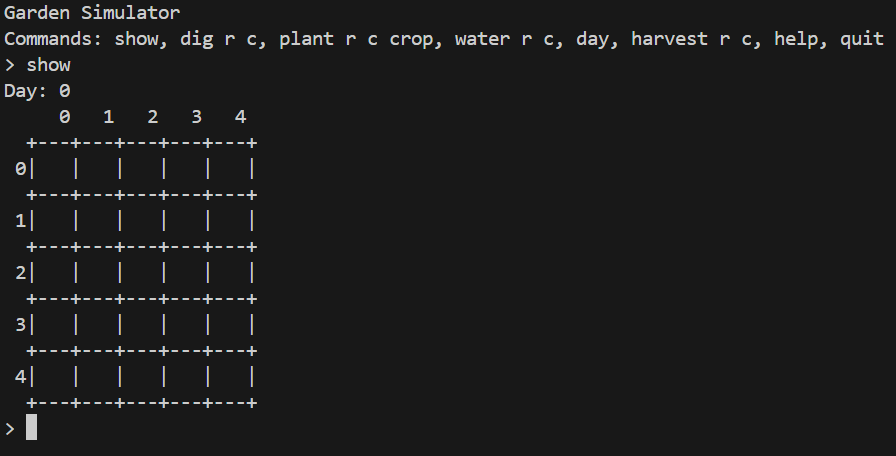
\includegraphics[width=0.8\textwidth]{00_figures/garden-sim.png}
  \caption{Startansicht des Garden-Simulators mit ausgeführtem show-Befehl}
  \label{fig:garden-sim}
\end{figure}


\subsubsection{README.md als Informationsquelle}

\subsection{Programmstruktur des \anf{Garden-Simulators}}
Funktional bildet der Simulator einen festgelegten Handlungszyklus ab: Zuerst wird ein Feld gegraben, anschließend bepflanzt, danach regelmäßig gegossen, die Zeit wird tageweise fortgeschritten und schließlich kann geerntet werden. Die Ausgabe erfolgt im Terminal als leicht lesbares Raster mit einfachen Symbolen, ergänzt um Zeilen- und Spaltenindizes, damit Interaktionen über Koordinaten nachvollziehbar bleiben. 

Diese Regeln sind in einer Zustandslogik definiert: 


\begin{itemize}
    \item Graben ist nur auf leeren Feldern möglich und erzeugt ein „hole“
    \item Pflanzen ist ausschließlich auf einem „hole“ erlaubt und erzeugt ein „seed“
    \item Gießen ist nur bei „seed“ oder „sprout“ zulässig und erhöht den Wasserstand bis zu einem Maximalwert
    \item Das Fortschreiten eines Tages wirkt auf alle Zellen gleichzeitig. Der Wasserstand wird pro neuem Tag um 1 verringert.
    \item Ernten ist wiederum nur im Zustand „ripe“ möglich
\end{itemize}

Die in Abb. \ref{fig:garden-sim-aufbau} gezeigte Repository-Struktur trennt klar zwischen Kernlogik, Darstellung und Interaktion. In garden.py liegt die zentrale Logik als Sammlung von Funktionen; dort werden gezielt Stubs mit Docstrings, Kommentaren und Beispielen bereitgestellt, die zunächst noch nicht implementiert sind und teils NotImplementedError auslösen. In cli\_view.py befindet sich eine vorgegebene, von Studierenden nicht zu verändernde Hilfsklasse (GardenPrinter), die den Garten ausschließlich liest und als Text darstellt; dadurch wird eine konsistente Visualisierung sichergestellt, ohne dass Studierende bereits objektorientierte Konzepte benötigen. main.py stellt eine einfache Kommandozeilen-Interaktion bereit, in der Befehle wie \texttt{dig r c}, \texttt{plant r c crop}, \texttt{water r c}, \texttt{day}, \texttt{harvest r c} oder \texttt{show} eingegeben werden können. Das Parsing erfolgt bewusst mit String split und if/else, um den Fokus auf Kontrollstrukturen, Zustandsprüfungen und Datenmanipulation zu legen.

\begin{figure}[htbp]
  \centering
  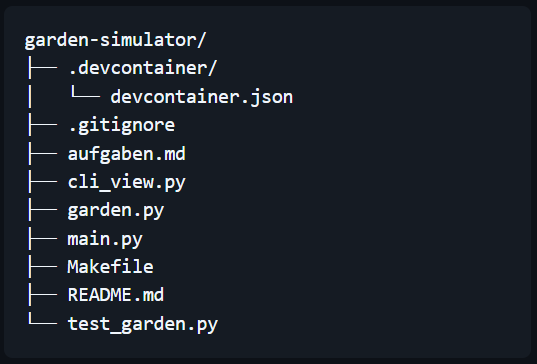
\includegraphics[width=0.5\textwidth]{00_figures/garden-sim-struc_2.png}
  \caption{Repository-Aufbau des \anf{Garden-Simulators}}
  \label{fig:garden-sim-aufbau}
\end{figure}

In test\_garden.py sind unter Zuhilfenamhe des pytest-Frameworks Unit-Tests hinterlegt, die für jede Funktion konkret festlegen, welches Verhalten erwartet wird wie z. B. erlaubte Zustandswechsel, Rückgabewerte oder out-of-bounds-Fälle. Für Studierende dienen diese Tests als verlässliche Referenz, weil sie nach jeder Implementationsänderung sofortiges, objektives Feedback liefern und typische Fehler klar sichtbar machen. Gleichzeitig bilden die Tests eine transparente Grundlage für die Auswertung. Wenn das Programm alle Tests besteht, erfüllt es Level 4 der Kategorie \enquote{Funktionaliät und Robustheit} des Bewertungsrasters in Tabelle \ref{tab:bewertungsrasterV2}.

\subsection{Erstellung der Aufgaben nach UMC-Framework}\label{cha:Aufgabenstellung}
Als Programmieraufgabe sollen die Studierenden in der bestehenden Python CLI-Anwendung \textit{Garden-Simulator} bestimmte Use Cases implementieren. Das didaktische Design dieser Unterrichtseinheit basiert auf dem Use-Modify-Create (UMC) Framework, wie es ursprünglich von \textcite{lee_umc_2011} definiert wurde. Empirische Studien, wie die von \textcite[S.~400]{lytle_use_2019} zeigen, dass dieser Ansatz insbesondere ab der Modify-Phase zum einen die Identifikation mit dem selbst geschriebenen Code (Ownership) stärkt. Zum anderen und für diese Arbeit wichtiger wird auch die Überforderung bzw. die kognitve Last auf Studierendenseite reduziert.

Die Programmieraufgabe ist in die drei Phase des UMC-Frameworks aufgeteilt. In der ersten Phase (Use) geht es um das Kennenlernen und Ausführen des Source Codes. Im Fall des Garden-Simulators sollen auch einfach Commands in das Command Line Interface (CLI) eingegeben und ausgeführt werden. Die zweite Phase fordert von den Studierenden, den in Phase 1 genutzten Code iterativ anzupassen. Um den Code gezielt zu verändern, muss auf Seite der Studierenden zumindest Teile der inneren Logik durchdrungen worden sein. Die dritte und finale Phase besteht aus der Erweiterung des bestehenden Artefakts. Die Studierenden fügen hier weitesgehend eigenständig eine neue Funktion hinzu. Was zu implemtieren ist, wird aufgrund der begrenzten Zeit verbal vorgegeben, auf eine zu detaillierte Aufgabenbeschreibung oder Hinweise im Code wurden jedoch verzichtet. \parencite{lee_umc_2011}.

Die folgenden Aufgaben sind von den Studierenden zu implementieren. 
\begin{enumerate}
  \item Führe den \texttt{help} command aus und sehe dir die Liste an Commands an. Gehe einen Harvest-Zyklus für das Crop \enquote{tomato} in der CLI durch. Führe dafür folgende Commands aus: \texttt{dig}, \texttt{plant}, \texttt{water}, \texttt{day}, \texttt{water}, \texttt{day}, \texttt{water}, \texttt{day}, \texttt{harvest}.
  \item Für den Command \texttt{quit} fehlt die Beschreibung im help-Befehl. Füge
  \begin{enumerate}
    \renewcommand{\labelenumii}{\roman{enumii}.}
    \item \enquote{quit} als Command-Name hinzu,
    \item \enquote{Exit the simulator} als Beschreibung und
    \item \enquote{quit} als Beispiel.
  \end{enumerate}
  \item Wenn eine Tomate geerntet wird, wird eine Datei names tomato.txt erstellt. Der User soll über das Erstellen der tomato.txt informiert werden. Der Satz \enquote{Created file 'tomato.txt' at <current datetime>} soll in der Konsole ausgegeben werden. Die Aufgabe ist im Code mittels Kommentarblöcken markiert.
  \newline
  Beispiel:
  \newline
  \texttt{Created file 'tomato.txt' at 18.05.2026 18:36:22.}

  \item Wenn keine Tomate geerntet wird, soll bei den anderen Crops in der Konsole der Satz ausgegeben werden: \enquote{[Info] The crop <name of the crop> has no file entry.}
  \newline
  Beispiel:
  \newline
  \texttt{[Info] The crop carrot has no file entry.}

  \item Füge ein neues Crop \enquote{potato} hinzu. Man soll es schon nach 2 \texttt{water} + \texttt{day} Zyklen ernten können. Die Aufgabe ist im Code nicht mittels Kommentarblöcken markiert. Es müssen dazu Änderungen in beiden Dateien main.py und garden.py gemacht werden.

\end{enumerate}

\subsection{Musterlösung der Aufgaben und Programmierkonzepte}
TODO, todo


\subsection{Lokale Tests zur Selbstüberprüfung}\label{cha:test-runner}

Um herauszufinden, ob die jeweilige Teilaufgabe korrekt erledigt wurde, können die Studierenden mittels des Commands \texttt{python test\_runner.py} lokale Tests ausführen. Ein Report über bestandene und nicht bestandene Testcases, wie in Abb. \ref{fig:test-runner-results} dargestellt, wird im Terminal präsentiert. Die Tests sollen den Programmier-Prozess der Studierenden unterstützen und so einerseits die korrekte Erledigung einer Aufgabe validieren und andererseits als Debugging-Instrument dienen. Letzteres, also das Lösen einzelner Probleme oder Fehler im Code, ist nach \textcite[S.~26]{edwards_using_2004} ProgrammiereinsteigerInnen besonders zeitintensiv und resultiert oft in wahllosen Herumprobieren. Idealerweise sollten die Tests von den Studierenden im Rahmen des Test Driven Developments selbst verfasst werden \parencites[S.~27--28]{edwards_using_2004}[S.~532--533]{janzen_test-driven_2008}. In der vorliegenden Arbeit werden die Tests hingegen aufgrund der begrenzten Bearbeitungszeit bereitgestellt.

\begin{figure}[htbp]
  \centering
  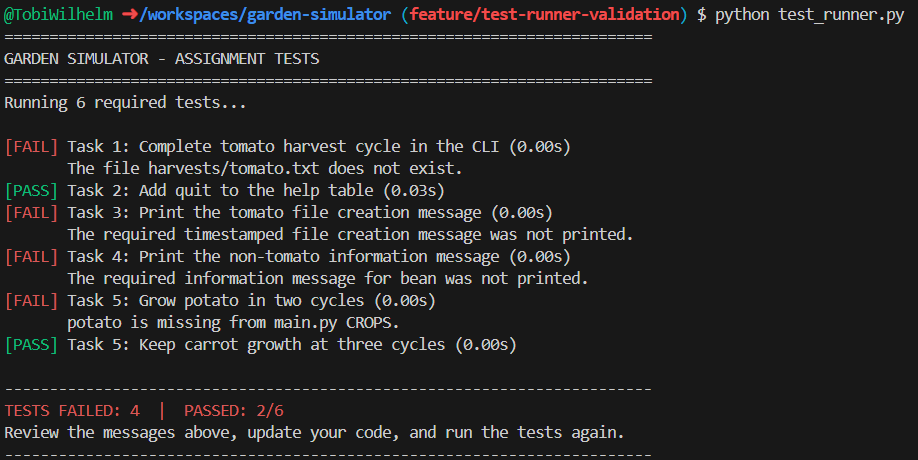
\includegraphics[width=0.8\textwidth]{00_figures/test-runner-false.png}
  \caption{Ausgabe des lokalen Testrunners bei fehlgeschlagenen und bestandenen Tests}
  \label{fig:test-runner-results}
\end{figure}

Wie in Abb. \ref{fig:test-runner-results} zu sehen ist, gibt es für jede Teilaufgabe einen eigenen Test. Als Hilfestellung und um den Testcase zu konkretisieren wird bei jedem fehlgeschlagenen Testcase ein Statustext ausgegeben. So wird z.B. für die nicht erfüllte Teilafgabe drei ausgegeben: \enquote{The required timestamped file creation message was not printed.} Für Teilaufgabe fünf gibt es jedoch zwei Tests. Denn, wie in der Aufgabenstellung in \ref{cha:Aufgabenstellung} erwähnt, müssen hier die benötigten \texttt{day}- und \texttt{water}-Zyklen bis zur Erntereife für das Crop \texttt{potato} adaptiert werden. Es kann hierbei aber passieren, dass die Zyklenanzahl auch für andere Crops verändert wird. Daher wird im letzten Testcase überprüft, ob für ein anderes Crop, in diesem Fall \texttt{carrot}, weiterhin die regulären drei \texttt{day}- und \texttt{water}-Zyklen bis zur Reife erforderlich sind.
